In dieser Seminararbeit soll eine spezielle Untermenge der Graphen un\-ter\-sucht werden, die sogenannten chordalen Graphen.

Chordale Graphen sind vor allem theoretisch interessant, da einige Probleme, die auf der Menge aller Graphen NP-vollständig sind, auf chordalen Graphen nur lineare Zeit benötigen. Dazu zählt beispielsweise das \textsc{Clique}-Problem (Entscheide für einen Graphen \( G = \left( V, E \right) \) und eine Zahl \( k \), ob es eine Knotenmenge \( X \subseteq V \) gibt mit \( \left| X \right| = k \), deren induzierter Teilgraph \( G \left[ X \right] \) vollständig ist).\footnote{siehe \cite[Satz 4.17]{golumbic}}%;  für den Satz\cite[Kapitel 13.2]{hagerup} für die Definition von \textsc{CLIQUE}}

\begin{definition}[Chordaler Graph]
	Sei \( G = \left( V, E \right)\) ein ungerichteter Graph.\linebreak{}
	\( G \) ist chordal, wenn jeder Kreis mit mindestens \( 4 \) Knoten eine Sehne (englisch: chord, also eine Kante zwischen zwei auf dem Kreis nicht-benachbarten Knoten) besitzt.\footnote{siehe \cite[Kapitel 4.1]{golumbic}}
\end{definition}

Ein Beispiel für einen chordalen Graphen ist in Abbildung \ref{fig:chordalgraph} (ohne die gestrichelte Kante) zu sehen. Würde man die gestrichelte Kante hinzunehmen, wäre \( \left( v_0, v_1, v_2, v_5, v_0 \right) \) ein Kreis mit vier Knoten ohne Sehne -- und somit wäre der Graph nicht mehr chordal.

\vspace{1em}
\begin{minipage}{\linewidth}
	\centering
	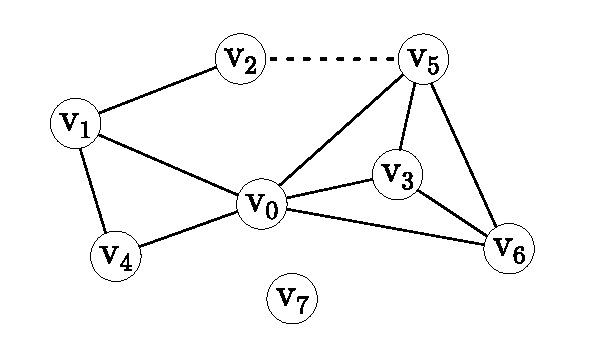
\includegraphics[scale=0.9]{img/graph/chordal.pdf}
	\captionof{figure}[Chordaler Graph]{Der hier abgebildete Graph \( G \) (ohne die gestrichelte Kante) ist chordal.}
	\label{fig:chordalgraph}
\end{minipage}

